\pagebreak
\section{Verifica}
\label{sez:verifica}

La verifica è un'attività cruciale del ciclo di vita del \textit{software}, finalizzata a garantire che il prodotto sviluppato soddisfi i requisiti specificati e sia privo di errori o difetti.\\
Questa attività si concentra sul controllo della correttezza, della completezza e della qualità del \textit{software}, sia a livello di codice che di comportamento.\\

\noindent La verifica può essere suddivisa in due approcci principali:

\begin{itemize}
\item \textbf{Analisi statica}:
È un processo che analizza il \textit{software} senza eseguirlo. \\
Si basa su tecniche di analisi statica, come le revisioni manuali del codice, l'uso di strumenti automatici per il controllo delle regole di codifica o per il \textit{linting} del codice. \\
Questo approccio consente di individuare errori, violazioni di standard, vulnerabilità e problemi di stile a livello di codice sorgente.  

\item \textbf{Analisi dinamica}:
Si basa sull’esecuzione del \textit{software} per testarne il comportamento in ambienti controllati o reali.\\
Questo approccio verifica che il sistema funzioni correttamente con \textit{input} specifici e che produca gli \textit{output} attesi. \\
Include attività come i \textit{test} unitari, \textit{test} di integrazione e \textit{test} di sistema.  
\end{itemize}

\noindent L’utilizzo combinato di analisi statica e dinamica è essenziale per garantire un livello elevato di qualità del \textit{software}. \\

\subsection{Analisi statica}
\label{subsec:analisi-statica}

Ho effettuato analisi statica per garantire che il codice sviluppato fosse conforme agli standard di qualità richiesti, riducendo la possibilità di errori e migliorandone la leggibilità e la manutenibilità.\\
Per questa attività ho utilizzato strumenti consolidati come \textit{Prettier} ed \textit{ESLint}, configurati per integrarsi con il flusso di lavoro del progetto.\\

\subsection{Analisi dinamica}
\label{subsec:analisi-dinamica}


Ho effettuato analisi dinamica per verificare il corretto funzionamento delle diverse componenti del sistema, concentrandomi in particolare sul \gls{backend}, considerato il cuore del progetto. \\
Il testing sul \gls{frontend} è stato affrontato in una fase successiva, con un approccio meno approfondito rispetto a quello dedicato al \gls{backend}.\\

\noindent Di seguito, descrivo in dettaglio le attività di \textit{testing} dinamico effettuate sia sul \gls{frontend} che sul \gls{backend}.
\pagebreak
\subsubsection{\textit{Testing} del \gls{backend}}

Ho sviluppato \textit{test} unitari per tutti i \textit{controller} e i \textit{service}, assicurando una copertura completa delle funzionalità fondamentali del sistema.\\

\noindent Durante l'intero ciclo di vita del \textit{software}, ho adottato il modello a \textit{V} (illustrato in {\hyperref[fig:v-model]{Figura 3.8}}), che integra il \textit{testing} sin dalle attività iniziali dello sviluppo. \\
Con un approccio iterativo, per ogni \textit{endpoint} creato ho immediatamente sviluppato i relativi \textit{test}, garantendo così la loro correttezza.\\

\noindent In totale, ho implementato 70 \textit{test} unitari nel \gls{backend}, coprendo una vasta gamma di funzionalità chiave del sistema.\\
Ho dedicato particolare attenzione alla funzionalità di generazione dei progetti tramite \gls{llm}, che rappresenta una parte cruciale del flusso di lavoro dell'applicazione.\\
 Questa funzionalità, infatti, è essenziale per la creazione automatizzata dei progetti e per garantire l'integrità dei dati generati.\\

\noindent Per simulare un ambiente di \textit{test} il più realistico possibile, ma senza dipendere direttamente dalle risorse esterne, ho creato dei \textit{mockup} per simulare il comportamento di funzionalità critiche.\\
In particolare, ho sviluppato \textit{mockup} per le interazioni con i servizi \textit{AWS Bedrock} e \textit{AWS S3}, utilizzati rispettivamente per la chiamata ai modelli di linguaggio e per la gestione dei documenti.\\
Questi \textit{mockup} hanno permesso di replicare il comportamento atteso di questi servizi, consentendo il \textit{testing} senza richiedere accesso diretto a tali risorse esterne.\\

\noindent Questo approccio ha permesso di testare e validare ogni componente sin dalla sua creazione, riducendo al minimo i rischi di errori e facilitando il \textit{debug} nelle attività successive di sviluppo.

\begin{figure}[H]
    \centering
    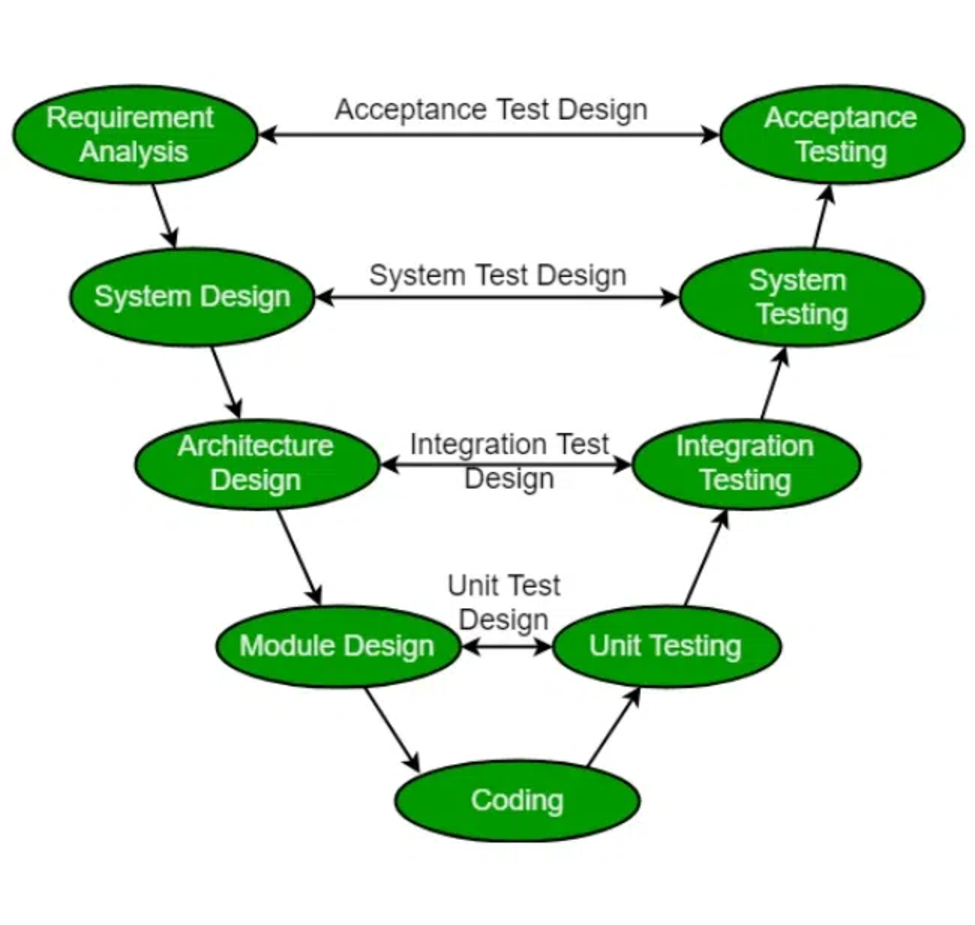
\includegraphics[scale=0.43]{v-model.png}
    \caption{Modello a V sviluppo \textit{software}}
    \label{fig:v-model}  
    \cite{site:v-model}
\end{figure}

\subsubsection{\textit{Testing} del \gls{frontend}}

Il \textit{testing} del \gls{frontend} è stato affrontato principalmente nell'ultimo \gls{sprint} del progetto, con un focus minore rispetto al \gls{backend}, in quanto le funzionalità del \gls{frontend} erano strettamente dipendenti dal corretto funzionamento del \gls{backend}.\\

\noindent Durante questo \gls{sprint}, il mio approccio si è concentrato principalmente sul \textit{test} delle funzioni logiche delle pagine, così come sulle chiamate \gls{api}, per assicurarmi che i dati venissero correttamente recuperati e visualizzati.\\
Le chiamate \gls{api} sono state verificate per garantire che rispondessero correttamente in termini di formati e tempistiche.\\

\noindent In totale, ho implementato 32 \textit{test} unitari per il \gls{frontend}, includendo sia le logiche delle pagine che la gestione delle chiamate alle \gls{api}.\\
Inoltre, ho utilizzato \textit{React Testing Library} per eseguire \textit{test} sui singoli componenti, in modo da verificarne la corretta visualizzazione e interazione con l'utente. \\
Questo strumento mi ha permesso di testare i componenti in modo isolato, simulando gli eventi utente (come i \textit{clic} e la compilazione di moduli) e controllando la corretta risposta da parte dell'interfaccia utente.\\

\noindent Il \textit{focus} del \textit{testing} del \gls{frontend} è stato limitato rispetto a quello del \gls{backend}, ma ha comunque permesso di garantire che l'interfaccia utente rispondesse correttamente alle azioni degli utenti e che tutte le chiamate alle \gls{api} si comportassero come previsto.


\subsubsection{\textit{Test} di rendimento}  

Nel corso dello sviluppo, ho dedicato particolare attenzione alla valutazione delle prestazioni del \gls{backend}, eseguendo una serie di \textit{test} di rendimento focalizzati sulla funzionalità di generazione dei progetti, che rappresenta una delle operazioni più critiche del sistema. \\

\noindent Questi \textit{test} sono stati progettati per misurare in dettaglio i tempi di risposta del sistema durante la creazione di un progetto, al fine di garantire che le operazioni avvenissero in maniera tempestiva e senza ritardi significativi. \\
Ho esaminato vari scenari, inclusi i casi in cui il sistema gestisce grandi quantità di dati, per assicurarmi che fosse in grado di rispondere in modo efficiente anche in situazioni di carico moderato.\\

\noindent Inoltre, i \textit{test} hanno incluso simulazioni di più richieste simultanee, per analizzare come il sistema si comportasse in scenari di stress e per verificare che non ci fossero colli di bottiglia o rallentamenti significativi durante il picco di utilizzo. \\

\noindent Questi \textit{test} di rendimento sono stati fondamentali per assicurare che il \gls{backend} fosse non solo funzionale, ma anche scalabile e in grado di gestire l'elaborazione di progetti in modo efficiente, riducendo i rischi di inefficienze o interruzioni delle prestazioni durante l'uso del sistema.
